\documentclass{standalone}
\usepackage{pgf, tikz}
\usepackage{mathtools}
\usetikzlibrary{arrows, automata}

\begin{document}

    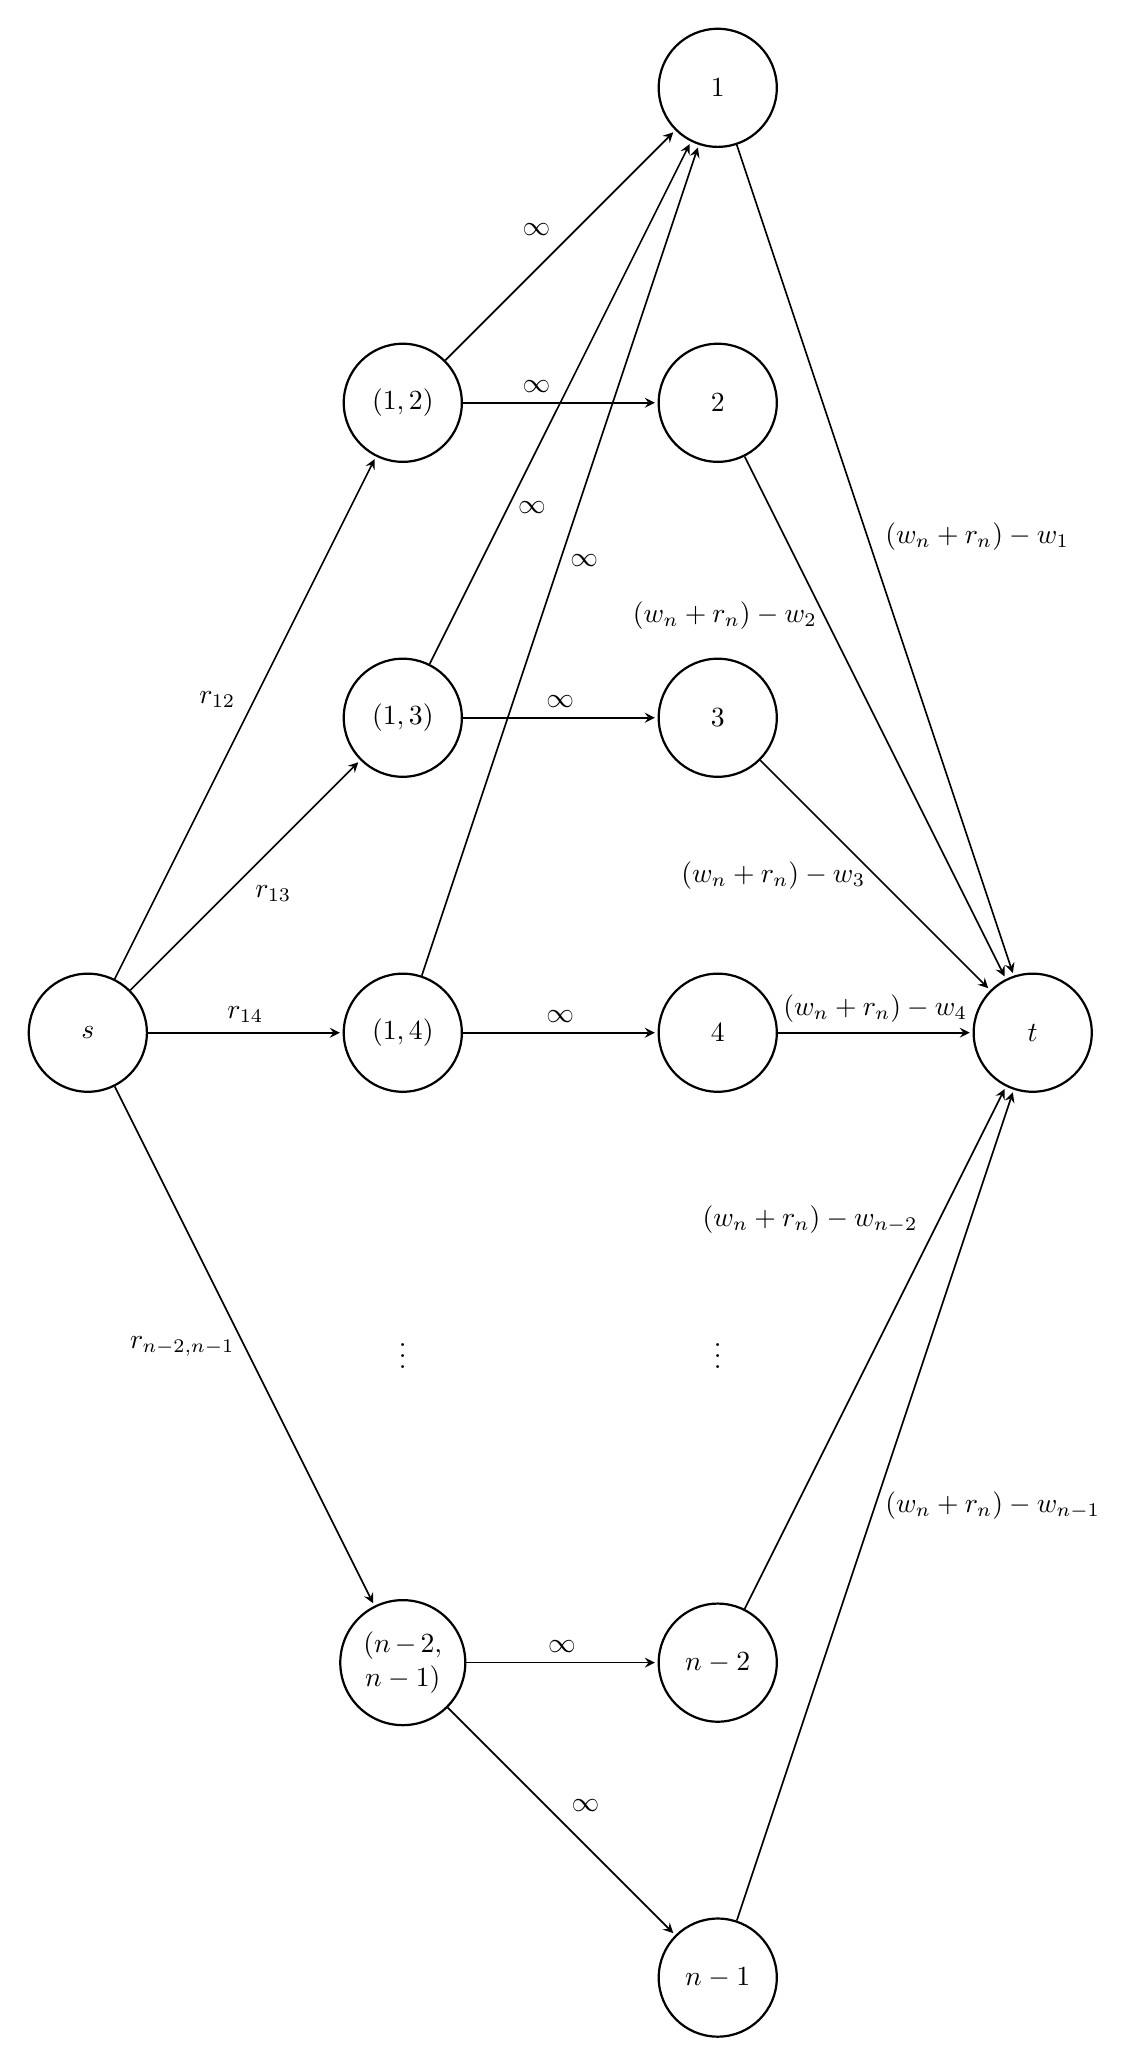
\begin{tikzpicture}[
            > = stealth, % arrow head style
            shorten > = 1pt, % don't touch arrow head to node set to +pt
            auto,
            node distance = 40mm, % distance between nodes
            semithick % line style
        ]

        \tikzstyle{every state}=[
            draw = black,
            thick,
            fill = white,
            minimum size = 15mm,
            text width = 10mm,
            align = center
        ]

        \node[state] (s) {$s$};

        \node[state] (t3) [right of=s] {$(1,4)$};
        \node[state] (t2) [above of=t3] {$(1,3)$};
        \node[state] (t1) [above of=t2] {$(1,2)$};
        \node[state, draw=white] (td) [below of=t3] {$\vdots$};
        \node[state] (tn1) [below of=td] {$(n-2,$\\$n-1)$};

        \node[state] (e4) [right of=t3] {$4$};
        \node[state] (e3) [above of=e4] {$3$};
        \node[state] (e2) [above of=e3] {$2$};
        \node[state] (e1) [above of=e2] {$1$};
        \node[state, draw=white] (e5) [below of=e4] {$\vdots$};
        \node[state] (e6) [below of=e5] {$n-2$};
        \node[state] (e7) [below of=e6] {$n-1$};

        \node[state] (t) [right of=e4] {$t$};


        \path[->] (s) edge node {$r_{12}$} (t1);
        \path[->] (s) edge node[below right] {$r_{13}$} (t2);
        \path[->] (s) edge node {$r_{14}$} (t3);
        \path[->] (s) edge node[left] {$r_{n-2,n-1}$} (tn1);

        \path[->] (t1) edge node {$\infty$} (e1);
        \path[->] (t1) edge node[above left] {$\infty$} (e2);
        \path[->] (t2) edge node[pos=0.3, right] {$\infty$} (e1);
        \path[->] (t2) edge node {$\infty$} (e3);
        \path[->] (t3) edge node[right] {$\infty$} (e1);
        \path[->] (t3) edge node {$\infty$} (e4);
        \path[->] (tn1) edge node {$\infty$} (e6);
        \path[->] (tn1) edge node {$\infty$} (e7);

        \path[->] (e1) edge node {$(w_n + r_n) - w_1$} (t);
        \path[->] (e2) edge node[pos=0.35, above left] {$(w_n + r_n) - w_2~$} (t);
        \path[->] (e3) edge node[left] {$(w_n + r_n) - w_3$} (t);
        \path[->] (e4) edge node {$(w_n + r_n) - w_4$} (t);
        \path[->] (e6) edge node[pos=0.7] {$(w_n + r_n) - w_{n-2}$} (t);
        \path[->] (e7) edge node[right] {$(w_n + r_n) - w_{n-1}$} (t);

    \end{tikzpicture}

\end{document}
